\section{Application au traitement du langage écrit}
\subsection{Introduction}
\subsubsection{La loi de Zipf et Mandelbrot}
Au $20^{ieme}$ siècle, Zipf proposa une loi, nommée \textit{Loi de Zipf} pour expliquer la fréquence d'apparition d'un mot au sein d'un texte (volumineux). Selon cette loi, si $mot^n$ est le $n^{ieme}$ mot le plus fréquent, alors sa fréquence d'apparition est définie par $Z(n)=\frac{K}{n}$ avec K, une constante. Supposons K=1, alors la fréquence de ce mot est de $\frac{1}{n}$.\\

\noindent Pour rappel, la Figure \ref{zipf} illustre son comportement pour K=1. Nous pouvons observer que la répartition statistique des mots est très fortement déséquilibrée. Des mots sont omniprésents alors que d'autres sont quasi-absents. Ce comportement justifie des difficultés historiques du traitement du langage naturel car les modèles reposant sur des fondations statistiques, cette particularité constitue une contrainte importante. Une seconde interrogation se porte sur la nature des mots fréquents et peu fréquents. Il a été montré que les mots récurrents sont des mots de liaisons grammaticales (adverbes, pronoms, déterminants...) alors que les mots illustratifs (noms, adjectifs...) sont plus rares. Cette particularité accentue la difficulté d'analyse car l'information discriminante est \textit{rare}.\\

\noindent Dans les faits, la loi de Zipf est incomplète et a été généralisée par Mandelbrot. En effet, Zipf a été vivement critiqué pour avoir exploité des mots non \textit{lemmatisés}\footnote{Cette notion est explicitée dans la suite de cette introduction}. La loi de Mandelbrot est ainsi définie par $M(n)=\frac{K}{(a+bn)^{c}}$ avec a,b,c et K des constantes.\\

\noindent Cette loi illustre des problématiques récurrentes en traitement du langage. Le comportement statistiques des données soulève des contraintes mathématiques notamment des biais pour manque de représentativité\footnote{Des mots peuvent ne pas être représentés dans les données d'apprentissage par exemple, ce qui est très délicat à exploiter pour les approches probabilistes}. La faible proportion de mots explicatifs nuit aux capacités de discrimination des modèles et les rend plus sensible au bruit des données d'apprentissage. Le traitement du langage naturel (\textit{Natural Language Processing}) est, aujourd'hui encore, un problème partiellement résolu et la recherche toujours fortement active.

\begin{figure}
\centering
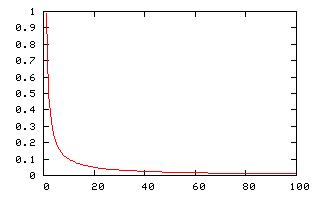
\includegraphics[scale=0.4]{./tex/natural-language-processing/zipf.png}
\caption{Loi de Zipf pour K=1}
\label{zipf}
\end{figure}

\subsubsection{Pré-traitement d'un texte}
Afin d'exploiter une donnée textuelle, deux catégories de pré-traitement sont nécessaires. La première consiste à \textit{normaliser} le texte afin de considérer une forme qui facilite l'apprentissage et limite le bruit intrinsèque lié à une distribution de données peu exploitable. La seconde permet de représenter un texte dans un format compréhensible par un réseau neuronal. En effet, seules les valeurs numériques sont exploitables. Il est donc nécessaire de trouver une approche permettant de représenter une valeur textuelle (donc catégorielle) en valeur numérique.

\paragraph{Tokenization}
Un réseau de neurones exploite des séquences de valeurs (série de pixels dans le cadre d'une image par exemple). Afin d'exploiter un texte, il est nécessaire de rendre son architecture sérielle, i.e transformer un texte en une suite d'entités de même nature. La Tokenization est le procédé qui permet de réaliser cette tâche. Lors de la Tokenization, une entité unitaire est appelée \textit{Token}.\\

\noindent \textbf{Important}: Dans la suite de cette introduction, nous considérerons l'alphabet latin. Bien que le raisonnement soit identique pour toutes les langues, les conclusions peuvent variées selon les spécificités de chacune.\\

\noindent Considérons un texte quelconque. Quelles sont les entités qui le constituent ?\\

\begin{tabular}{|c|c|}
    \hline
     Source &  Entité sous-jacente\\
     \hline
     Texte intégral & Phrases\\
     \hline
     Phrases & Mots\\
     \hline
     Mots & Syllabes\\
     \hline
     Syllabes & Lettres\\
     \hline
\end{tabular}
\bigbreak
\noindent Nous observons différentes catégories d'entités fondamentales. Dans les faits, un consensus a choisi le mots comme type de Token. Néanmoins, dans le cadre de certaines problématiques, plusieurs types de Tokenization peuvent être exploités\footnote{Ceci sera développé dans la suite de cette introduction.}.\\

\noindent Bien qu'en apparence simple, la Tokenization présente des difficultés notables dont la solution relève essentiellement d'une sensibilité personnelle plus que d'une approche scientifiquement démontrable. Parmi ces difficultés, nous pouvons citer l'exploitation de la ponctuation et des symboles (y compris les jeux graphiques tels que les \textit{émoticônes} par exemple), l'interprétation des mots composées et/ou à particules ou encore les ambiguïtés syntaxiques (notamment liées à l'apostrophe). De même, pour l'anglais, l'interprétation des contractions pose des difficultés. Comment traiter \textit{aren't} ? Par \textit{aren't, arent, aren t, are n't} ?\\

\paragraph{Lemmatisation et racinisation - A FAIRE}
En cours
\paragraph{Stopwords}
Lors d'une tâche de classification (Analyse sentimentale, catégorisation de documents par exemple), il est nécessaire d'extraire l'information discriminante d'un texte afin de pouvoir le classifier. Pour cela, il est nécessaire de mettre en valeur, les mots porteurs d'informations.\\

\noindent Les mots les plus fréquents dans un texte sont des entités de liaisons grammaticales. Par exemple, nous pouvons citer les déterminants, pronoms ou encore certains adverbes. Ces mots n'ont pas de pouvoir de discrimination car leur expression est neutre et/ou sont trop représentés statistiquement pour être discriminant. Par exemple, le mot \text{le} n'a aucun pouvoir de discrimination alors que l'auxiliaire \text{être} est trop représentés pour être discriminant. \\

\noindent Ces mots sont définis comme \textit{StopWords}, i.e des mots au pouvoir de discrimination nul. Ils sont donc inutiles pour la tâche de classification qui repose sur des entités au fort pouvoir explicatif. Une approche classique de pré-traitement de texte est donc de supprimer ces mots des textes à analyser pour ne conserver que des mots pertinents. \\

\noindent Ainsi, par exemple, supposons les tokens suivants: [Cet, article, est, une, arnaque, car, la, qualité, semble, mauvaise !]. Après suppression des \textit{StopWords}, nous obtenons : [article, arnaque, qualité, semble\footnote{Il est possible de discuter sur la pertinence ou non de ce mot.}, mauvaise].\\

\noindent Cette approche supprime les mots sans incidence sur la décision du réseau. La prédiction est donc plus rapide car le volume de données traitées est grandement diminué\footnote{Dans le cadre d'analyse intégrale d'oeuvres ou de documents} et l'apprentissage plus performant grâce à la plus grande spécialisation des données d'apprentissage. Néanmoins, cette méthode ne conserve pas la sémantique du texte ni sa structure syntaxique.

\paragraph{Problématique et pré-traitement}
Toutes les modifications précédentes (sauf Tokenization) détériorent l'intégrité sémantique et syntaxique d'un texte. Pour certaines tâches, cette détérioration est sans importance. Dans le cas d'une classification par exemple, cette perte a souvent des conséquences négligeables sur la qualité du résultat. Au contraire, pour les problématiques qui demandent de conserver une bonne structure sémantique et syntaxique, appliquer cette approche fera échouer l'apprentissage de manière critique. Il est donc important d'étudier les caractéristiques du problème à résoudre avant d'appliquer un pré-traitement sur les données.\\

\noindent Généralement, pour les tâches qui ne demandent pas de création de texte comme valeur de sortie, l'application de pré-traitement est envisageable. Nous pouvons citer l'analyse sentimentale, la Recherche d'informations, la désambiguïsation par exemple. Au contraire, lorsqu'un texte syntaxiquement cohérent doit être généré, utiliser un pré-traitement est dangereux. La traduction automatique, les systèmes Question-Réponse, les générateurs de texte ou encore l'Image Captioning sont des exemples classiques.\\

\noindent Néanmoins, les approches récentes de classification, notamment basées sur les RNN et les principes d'\textit{Attention} imposent la conservation de la structure sémantique et syntaxique du texte. De ce fait, le pré-traitement des données tend à devenir de plus en plus "néfaste" même sur des tâches qui s'y prêtent traditionnellement.

\subsection{Représentation vectorielle - A FAIRE}
% \subsubsection{One-hot vector}
% \paragraph{Term frequency-inverse document frequency (TF-IDF)}
 \subsubsection{Projection Word-Based - A FAIRE}
En cours
% \paragraph{Word2Vec}
% \paragraph{Glove}
% \paragraph{SENNA}
\subsubsection{Projection Character-Based}
En cours
% \paragraph{Deep Semantic Similarity Model (DSSM)}
\subsection{Classification}
La classification de texte est une thématique qui présente un fort intérêt d'un point de vue métier. Son objectif est, comme dans le cadre de l'image, de classer le texte dans une (ou plusieurs) catégorie qui correspond à ses spécificités. La classification des Tweets selon leurs "toxicités" (neutre, harcèlement, discrimination...) est un exemple classique d'application.\\

\noindent Cette thématique présente une grande diversité d'architecture exploitable. En effet, il est possible d'utiliser les réseaux convolutifs, les réseaux récurrents ou encore l'union de ces deux types de réseau. Nous verrons, dans cette partie, quelques unes des solutions standards de l'état de l'art et les spécificités théoriques observées dans le cadre de la classification de texte.\\

\noindent Aujourd'hui, il n'y a pas de consensus sur la meilleure famille d'architecture pour réaliser de la classification de texte. Néanmoins, les réseaux convolutifs sont plus rapides à apprendre et à réaliser des prédictions. Par contre, les réseaux récurrents ont une plus grande capacité de compréhension de la sémantique du texte, ce qui, dans le cas de texte difficile ou ambiguë, peut permettre de meilleurs résultats que les réseaux convolutifs.

\subsubsection{Classification par CNN}
\paragraph{CNN for Sentence Classification}
\textit{CNN for Sentence Classification}\cite{cnntxt1} est un modèle précurseur crée en 2014. Ce modèle considère le texte comme une séquence de mots et analyse les N-Grams obtenus selon les spécifités du filtre de convolution choisi. Cette approche néglige le contexte sémantique global du texte pour se focaliser sur le comportement local des groupes de mots.\\

\noindent Le réseau utilisé présente une architecture simple. Les Words Embeddings correspondant aux mots du texte sont générés aléatoirement ou issus d'une librairie de vecteurs pré-entraînés. Dans le cas où les vecteurs initiés sont pré-entraînés, la valeur des vecteurs est figée durant l'apprentissage. Il est possible de cumuler plusieurs Words Embeddings pour un même mot en concaténant les vecteurs. L'architecture du réseau applique une approche \textit{Inception}. Chaque flux exploite un kernel de dimension différente afin de produire différents N-Grams (le nombre de filtre est un hyper-paramètre). Il n'y a qu'une couche de convolution par flux. Le réseau est donc très peu profond mais large. Une couche de MaxPooling est appliquée sur chaque flux pour extraire les N-Grams les plus pertinents. Ces valeurs sont ensuite envoyées à une couche Full-Connected pour réaliser la prédiction. Le modèle est visible sur la Figure \ref{cnnsent}. \\

\noindent Ce modèle présente une efficacité convenable sur des textes simples et de petites tailles mais est insuffisant dans le cas contraire. Néanmoins, il mit en avant les capacités des réseaux convolutifs pour la classification d'un texte alors "dominé" théoriquement par les réseaux récurrents.

\begin{figure}
\centering
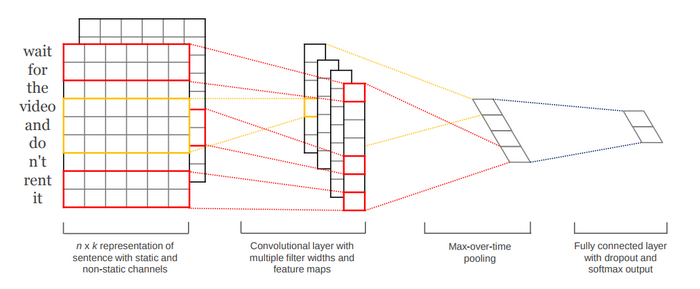
\includegraphics[scale=0.4]{./tex/natural-language-processing/cnnsent.png}
\caption{Architecture de CNN for Sentence Classification}
\label{cnnsent}
\end{figure}

\paragraph{Améliorations notables}
De nombreuses améliorations de \textit{CNN for Sentence Classification} ont été proposées. Néanmoins, l'architecture générale reste très similaire.
\begin{itemize}
    \item \textbf{Dynamic Convolutional Neural Network (DCNN)}\cite{dcnn}: Ce modèle exploite K-max Pooling pour capturer les relations courtes et longues distances dans le texte. Les kernels des couches de convolutions sont aussi plus larges et diminuent progressivement, de même que la dimension de sortie des couches de K-max Pooling. Son architecture est visible sur la Figure \ref{dcnn}.

    \item \textbf{Multi Channel Variable size CNN (MV-CNN)}\cite{multichannel}: Ce modèle est très similaire à \textit{Dynamic Convolutional Neural Network} mais exploite l'idée des Embeddings multi-sources. Ainsi, le modèle applique la même extraction d'attribut indépendamment pour chaque matrice initialisées par chacune des librairies d'Embeddings et réalise la prédiction à partir de la concaténation des résultats obtenus pour chaque flux\footnote{Si 2 librairies sont utilisées, il y aura deux flux.}. L'intuition repose sur le faits que les Words Embeddings sont définies selon des méthodes différentes mais surtout des jeux de données différents. Selon la source d'apprentissage, le contexte global peut changer et de ce fait, des mots rares ou absents dans une librairie peuvent être significatifs dans une autres. Son architecture est visible sur la Figure \ref{multichannel}. Une variante très proche, intitulé \textbf{Multi Group Norm Constraint CNN (MG(NC)-CNN)}\cite{multinorm}, repose sur une architecture similaire mais simplifiée en plus d'un ajout de contraintes de régularisation pour compenser la simplicité du modèle.

\end{itemize}

\begin{figure}
\centering
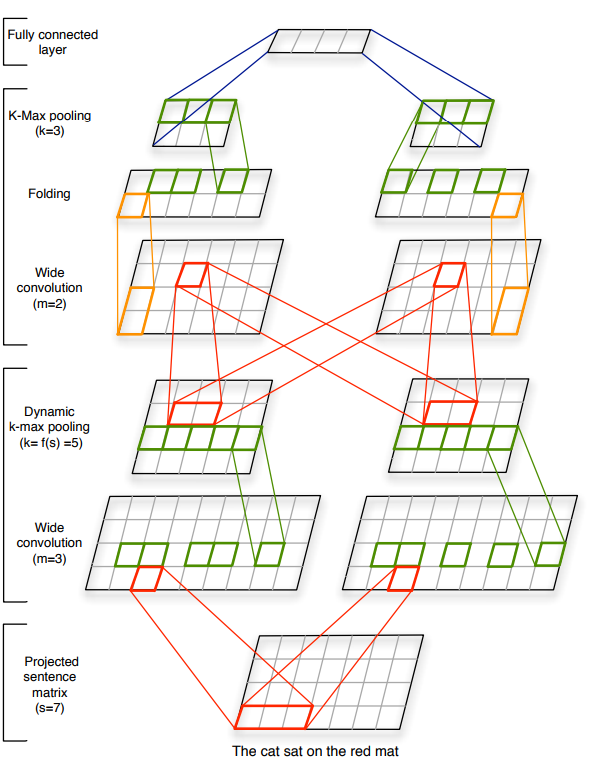
\includegraphics[scale=0.3]{./tex/natural-language-processing/dcnn.png}
\caption{Architecture de Dynamic Convolutional Neural Network}
\label{dcnn}
\end{figure}

\begin{figure}
\centering
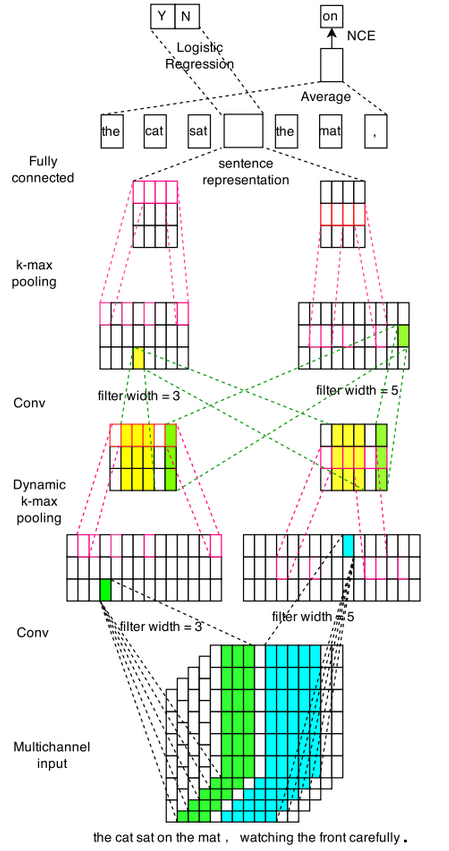
\includegraphics[scale=0.3]{./tex/natural-language-processing/multichannel.png}
\caption{Architecture de Multi Channel Variable size CNN}
\label{multichannel}
\end{figure}

\paragraph{Very Deep CNN}
Les modèles précédents se basent sur le mot comme unité de référence et exploitent un réseau peu profond mais large. Au contraire, \textit{Very Deep CNN} (VDNN)\cite{vdnn} exploite la lettre comme unité de référence et repose sur une architecture très profonde mais peu large. La ponctuation est les symboles sont considérés comme des lettres et utilisés par le réseau. Des projections vectorielles spécifiques aux lettres sont utilisées pour représenter chaque lettre. Afin de considérer la spécificité de l'unité choisie, le nombre de filtres est significativement augmenté mais la dimension du kernel reste dans le même ordre de grandeur (<5). Afin de progressivement diminuer la dimension des \ref{vdnn}.\\

\noindent Du fait de la profondeur du réseau et du volume de données à analyser, ce modèle est significativement plus lent à apprendre et à réaliser ses prédictions.

\begin{figure}
\centering
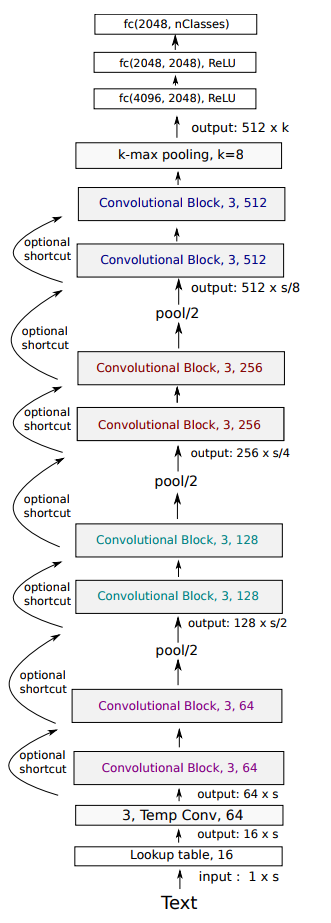
\includegraphics[scale=0.3]{./tex/natural-language-processing/vdnn.png}
\caption{Architecture de Very Deep CNN}
\label{vdnn}
\end{figure}

\paragraph{Comparatif expérimental sur les architectures CNN}
Deux études expérimentales ont été réalisées afin d'étudier les différentes approches et définir laquelle semble être la plus performante. \\

\noindent La première, réalisée par Hoa T. Le\cite{cnnsentexp}, a montré que dans le contexte de la classification de texte:

\begin{itemize}
    \item Les modèles larges et peu profonds sont meilleurs que les modèles très profonds. De plus, du fait de la complexité des modèles profonds, l'apprentissage de ce type de réseau est plus difficile et gourmand en temps et en ressources matérielles.

    \item L'utilisation de \textit{Global Max Pooling} avec un modèle peu profond mais large semble aussi performant que l'utilisation du \textit{Max Pooling} avec un modèle profond. La capacité très généralisante semble suffisamment discriminante dans le contexte de la classification.

    \item Les modèles exploitant le mot sont plus performants que les modèles basés sur la lettre. De plus, les modèles \textit{character-based} imposent l'exploitation d'un réseau très profond et de ce fait, s'associe aux problématiques de l'apprentissage et de ressources.
\end{itemize}

\noindent Ainsi, les réseaux de classification de textes s'opposent aux dogmes des réseaux de classification d'images qui reposent sur l'idée que le réseau doit être très profond pour être efficace.\\

\noindent La seconde étude, réalisée par Ye Zhang\cite{analysiscnn}, apporte une aide sur le paramétrage des hyperparamètres des modèles de classification de textes. Ainsi, plusieurs conseils ont été proposés:
\begin{itemize}
    \item Durant la première approche, exploitez des Word Embeddings non statiques\footnote{Variables durant l'apprentissage et non figés.} au lieu de \textit{One-Hot vector}. Concaténer plusieurs Word Embeddings ne semble pas améliorer significativement les performances de la classification.

    \item Exploitez une dimension de kernel entre 1 et 10. Réalisez éventuellement un \textit{GridSearch} autour de la meilleure valeur de kernel obtenue.

    \item Variez le nombre de filtres de 100 à 600. Durant la recherche, utilisez un DropOut (< 0.5) et une Max-Norm contrainte importante. Gardez en tête qu'il y a un compromis à faire entre nombre de filtres et temps d'apprentissage.

    \item Plus le nombre de \textit{feature map} au sein du réseau augmente, plus les contraintes de régularisation doivent être fortes.

    \item Ne pas négliger la Cross-Validation pour la recherche d'hyperparamètres pour éviter les biais d'apprentissage. Néanmoins, cette méthode est gourmande en temps de calculs.
\end{itemize}

\subsubsection{Classification par RNN}
Il existe des modèles de classification de textes basés sur les réseaux récurrents (spécialement avec des cellules LSTM ou GRU). Nous allons étudier plusieurs modèles de l'état de l'art reposant sur cette architecture.

\paragraph{LSTM Deep Sentence Embedding}
\textit{LSTM Deep Sentence Embedding}\cite{rnnsent} est un réseau simple à réaliser et présente des performances satisfaisantes. Il est composé d'un réseau LSTM-RNN et d'une couche Full-Connected qui exploite le vecteur d'états cachés de la dernière cellule LSTM. Ce vecteur résume l'information utile du texte analysé et de ce fait, représente un Embedding du document. Il utilise le mot comme entité-unité. La Figure \ref{lstmrnn} illustre l'architecture de ce modèle.\\

\noindent La faible dimension du vecteur caché permet de s'émanciper des couches de Pooling (ou autres méthodes de \textit{Downsampling}). Néanmoins, l'space de représentation est de faible dimension et de ce fait, favorise la perte d'informations. De plus, bien que le LSTM corrige grandement le problème de mémoire à long terme des réseaux récurrents, la perte d'informations dans le cas d'analyse de textes volumineux n'est pas à négliger.

\begin{figure}
\centering
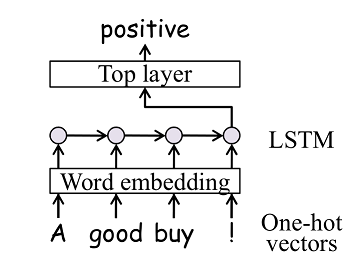
\includegraphics[scale=0.3]{./tex/natural-language-processing/lstmrnn.png}
\caption{Architecture de LSTM Deep Sentence Embedding}
\label{lstmrnn}
\end{figure}

\paragraph{Discriminative RNN}
\textit{Discriminative RNN}\cite{discrimi} est très similaire à \textit{LSTM Deep Sentence Embedding} mais propose une solution à la perte d'informations liée à la sélection du vecteur d'états cachés. Pour cela, au lieu d'exploiter le vecteur de la dernière cellule, l'Embedding du document sera égal à la moyenne des différents vecteurs d'états cachés du LSTM-RNN. Cette approche permet d'être moins sensible à la perte de mémoire liée à ce type de réseau. Son architecture est visible sur la Figure
\ref{discrimini}.

\begin{figure}
\centering
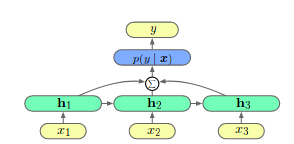
\includegraphics[scale=0.4]{./tex/natural-language-processing/discrimi.png}
\caption{Architecture de Discriminative RNN}
\label{discrimini}
\end{figure}

\paragraph{Hierarchical Attention Networks}
\textit{Hierarchical Attention Networks}\cite{hierarchical} pose le postulat qu'un mot et qu'une phrase ont deux pouvoirs explicatifs dissociés. Ainsi, afin de considérer ces deux sources d'informations, le réseau présente une architecture à deux niveaux composée de deux réseaux Bi-LSTM imbriqués. \\

\noindent Le premier niveau analyse le texte en isolant chacune des phrases et en analysant l'importance des mots qui constituent la phrase. Le second niveau analyse le texte en fonction des phrases dont l'information est calculée à travers le premier réseau. La sortie de ce réseau sera exploitée par la couche prédictive composée de couches Full-Connected.\\

\noindent Supposons un texte composé de N phrases et chacune des phrases possède M mots. Le premier réseau considérera une entrée composée de M éléments successifs et réaliseras N cycles prédictifs. Il produira donc N*M vecteurs d'états cachés (et N vecteurs d'états cachés finaux). Le second réseau considérera une entrée composé de N éléments successifs (chacun représentant l'information d'une phrase) et produira un cycle uniquement. Chaque entrée du second réseau correspond à la sortie obtenue à la fin d'un cyle du premier.\\

\noindent Cette architecture exploite aussi la notion d'\textit{Attention} (Voir Section \ref{softattention}). Ainsi, chaque entrée du second réseau correspond à une moyenne pondérée des vecteurs de contexte du premier réseau liés à cette entrée. La pondération est dynamique et apprise durant l'apprentissage. Cette méthode est aussi appliquée à la sortie du second niveau. Ce réseau est illustré par la Figure \ref{hierarchical}.


\begin{figure}
\centering
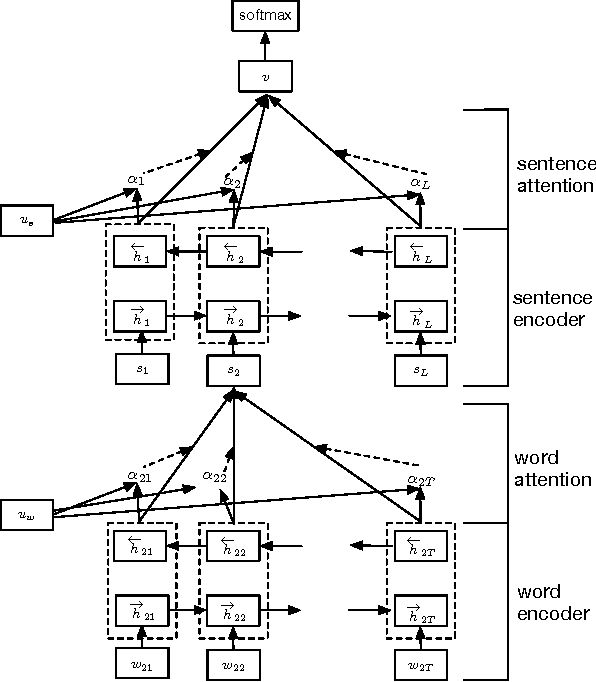
\includegraphics[scale=0.3]{./tex/natural-language-processing/hierachical.png}
\caption{Architecture de Hierarchical Attention Networks}
\label{hierarchical}
\end{figure}

\subsubsection{Classification par CNN-RNN}
Des architectures ont été développées en utilisant à la fois l'architecture CNN et RNN en se basant sur l'hypothèse que l'utilisation des deux architectures permettrait d'unir leurs points forts (compréhension sémantique du RNN et la détection de patterns locaux du CNN).\\

\paragraph{CNN-RNN}
\noindent Le modèle \textit{CNN-RNN}\cite{cnnlstm} est composé de deux parties:
\begin{itemize}
    \item \textbf{Extraction du vecteur de contexte}: Cette action est réalisée par un réseau convolutif (CNN). Ce réseau prend une séquence de \textit{Word Embeddings} en entrée et produit un vecteur représenté par la sortie d'une couche Full-Connected\footnote{La fonction d'activation de la couche est linéaire, i.e aucune fonction d'activation particulière n'est exploitée.}. Le réseau CNN présente une architecture peu profonde mais large comparable au réseau \textit{NN for Sentence Classification}.

    \item \textbf{Prédiction du label}: Cette action est réalisée par un réseau récurrent (RNN). Ce réseau exploite le vecteur de contexte pour initier son état caché initial en plus d'être additionné aux autres entrées des cellules RNN. L'addition suit la relation suivante:
    $$h^{(t)}=f_{activation}(W_hx_t+U_hh_{t-1}+W_TT)$$
    \noindent Avec T, vecteur de contexte et $W_T \in R^{q*t}$ avec q, dimension de l'état caché de la cellule RNN et t, dimension du vecteur de contexte.\\

    Une couche \textit{softmax} est appliquée en amont de chaque sortie du RNN afin de prédire le label le plus probable selon la sortie de la cellule RNN ciblée.\\

    La cellule RNN peut être remplacée par une cellule LSTM ou GRU afin de limiter l'impact de la perte de mémoire. Dans ce cas, le vecteur de contexte est ajouté à chacune des différentes \textit{Gates} de la cellule. La cellule n+1 utilise la prédiction faite par la cellule n-1, i.e son tag, afin d'orienter sa prédiction. Le réseau n'a connaissance du texte qu'à travers le vecteur de contexte proposé par le CNN. Il est donc important de s'assurer que la dimension de ce vecteur est suffisante pour représenter la séquence à prédire\footnote{Plus le texte est complexe et volumineux, plus la dimension du texte doit être grand. Néanmoins, l'utilisation de l'\textit{Attention} peut aider à éviter cette proportionnalité dimensionnelle.}. La Figure \ref{cnnrnn} illustre cette architecture.

\end{itemize}

\begin{figure}
\centering
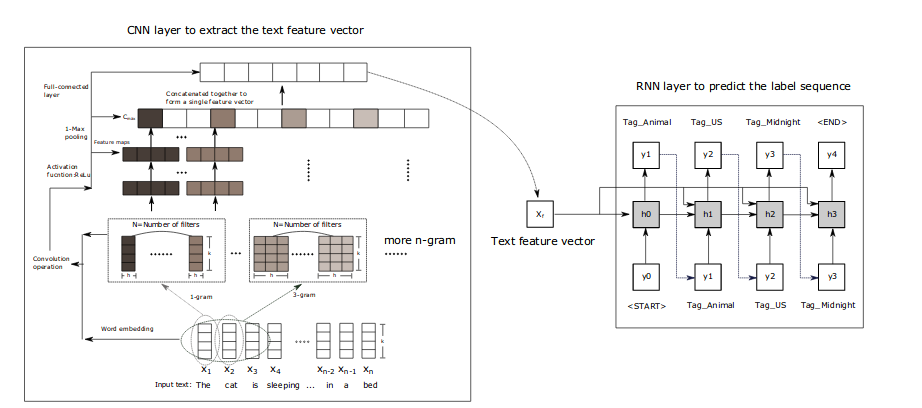
\includegraphics[scale=0.4]{./tex/natural-language-processing/cnnrnn.png}
\caption{Architecture de CNN-RNN}
\label{cnnrnn}
\end{figure}

\paragraph{C-LSTM}
\noindent Le modèle \textit{C-LSTM}\cite{clstm} est composé de deux parties:
\begin{itemize}
    \item \textbf{Extraction des N-Grams}: Le réseau convolutif applique n filtres (kernel identique) sur la séquence à prédire. Les n \textit{feature map} obtenus sont concaténés selon l'axe des colonnes. Le réseau présente deux particularités:
    \begin{itemize}
        \item Aucune méthode de Downsampling est utilisée (stride, Pooling...) afin de conserver la cohérence sémantique de la séquence\footnote{Extraire des sous-séquences détruit l'intégrité de la continuité sémantique}. Une alternative proposée par \cite{clstm2} reprend l'architecture du C-LSTM mais applique du Pooling afin de réduire la dimension des \textit{feature map} en sortie du réseau convolutif et ainsi, augmenter la vitesse de prédiction et d'apprentissage du réseau (voir Figure \ref{clst2m}).

        \item Un seul kernel est exploité afin de permettre une bonne concaténation et la cohérence des données concaténées. Néanmoins, exploiter différents kernels est possible en s'assurant du respect des dimensions des \textit{feature map} notamment via l'usage de \textit{padding}. \textbf{Cette spécificité est incertaine et relève de mon interprétation du papier de recherche. Veuillez vous référer au papier associé afin de confirmer cette affirmation}.
    \end{itemize}

    \item \textbf{Extraction d'un vecteur de contexte}: Le réseau RNN (LSTM) est utilisé afin d'interpréter le comportement sémantique du texte à partir des N-Grams obtenus par le réseau convolutif. Ainsi, l'entrée séquentielle i du RNN correspond aux N-Grams concatenés à la position i des différentes \textit{feature map}\footnote{Dans les faits, les \textit{feature map} sont représentées par une matrice unique de dimension i*j avec i nombre de N-grams et j, nombre de filtres. Les entrées du RNN correspondent donc aux lignes de la matrice.}.\\

    Une couche \textit{softmax} prend en entrée le \textbf{dernier état caché} du LSTM afin de réaliser sa prédiction. Il n'y a donc qu'une prédiction réalisée (à partir du dernier état caché) en fin de réseau alors qu'avec le modèle \textit{CNN-RNN}, la prédiction se fait \textit{en continu}à partir des différents états cachés du RNN.
\end{itemize}

\begin{figure}
\centering
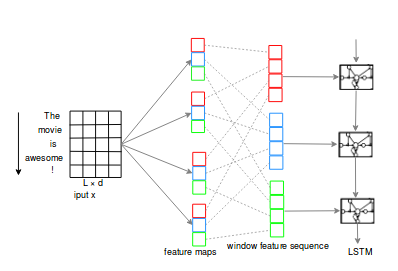
\includegraphics[scale=0.45]{./tex/natural-language-processing/clstm.png}
\caption{Architecture de C-LSTM}
\label{clstm}
\end{figure}

\begin{figure}
\centering
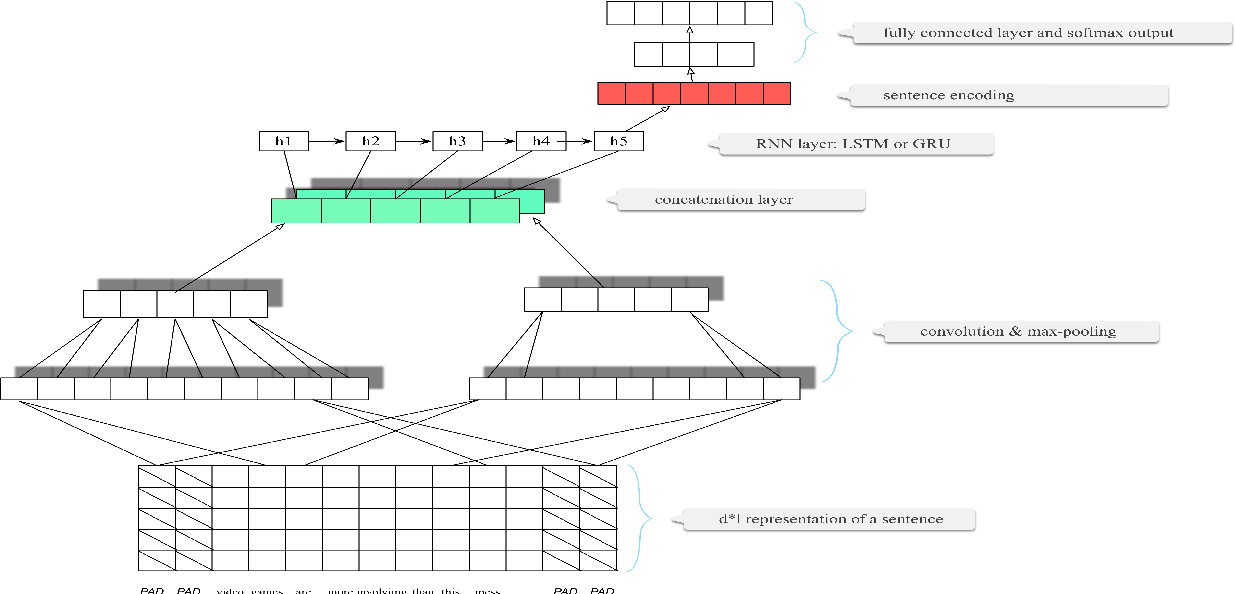
\includegraphics[scale=0.3]{./tex/natural-language-processing/clstm2.png}
\caption{Architecture de C-LSTM avec Pooling}
\label{clst2m}
\end{figure}

\paragraph{AC-BLSTM}
Le modèle \textit{symmetric Convolutional Bidirectional LSTM Networks} (AC-BLSTM) \cite{acblstm} propose une modification des couches convolutives nommée \textit{Asymmetric Convolution} afin d'extraire l'information de la séquence à prédire.\\

\noindent Supposons un séquence S de dimension L donc le j-ième mot $x_j$ est représenté par un \textit{Word Embeddings} tel que $x_j \in R^d$. Nous avons donc:
$$S=[x_1,...x_L]$$
$$x_i=[x_{i,1},...,x_{i,d}]$$

\noindent Supposons $k$ dimension du kernel du filtre d'une couche de convolution. Une convolution standard (sur une dimension) réalise donc une opération de dimension k*d, i.e analyse k mots successifs représentés par un vecteur de dimension d.\\

\noindent Une convolution asymétrique réalise la convolution en deux étapes convolutives:
\begin{itemize}
    \item La première étape est représentée par un kernel de dimension 1*d. Ainsi, l'action de cette opération correspond à une projection vectorielle définie par $R^d \longrightarrow R^1$. En d'autres mots, le \textit{Word Embeddings} est représenté par une valeur uniquement à la fin de cette étape.

    \item La seconde étape est représentée par un kernel de dimension k*1 où k correspond à la taille du filtre choisi initialement. Le fonctionnement de cette étape est comparable à une convolution standard sur des données à 1 dimension.
\end{itemize}

\noindent Expérimentalement, la convolution asymétrique a présenté des résultats qualitatifs. De même, on peut observer une ressemblance avec l'approche \textit{Depthwise-Pointwise} très utilisée pour l'analyse d'image et les réseaux faibles consommation.\\

\noindent La concaténation des \textit{feature map} et l'exploitation du réseau récurrent de AC-BLSTM est comparable à celle de C-LSTM. Deux différences importantes sont à notifier pour cette dernière.
\begin{itemize}
    \item Le réseau AC-BLSTM exploite un réseau \textit{Bi-directionnel} afin d'améliorer les capacités prédictives du réseau LSTM.

    \item La prédiction du label est réalisée à partir d'une couche softmax qui prend en entrée l'intégralité des états internes du BLSTM concaténés. Ainsi, supposons un réseau BLSTM composé de m cellules de dimension n. L'entrée de la couche softmax sera alors de dimension $m*(2*n)$.
\end{itemize}

\noindent Une illustration de l'architecture du réseau est visible sur la Figure \ref{acblstm}. Néanmoins, une particularité importante est à remarquer. Contrairement au réseau C-LSTM, AC-BLSTM accepte les kernels de tailles variables. Sans l'exploitation de padding, les \textit{feature map} sont de dimensions variables et ne peuvent être concaténées. Pour résoudre cette problématique, une méthode a été proposée.\\

\noindent Supposons un filtre de dimension $k_i$ appliqué sur une séquence de taille L, une convolution sans padding produira une \textit{feature map} de dimension $D_i=L-k_i+1$. Supposons maintenant un filtre de dimension $k_j$ tel que $k_j > k_i$ alors, la dimension de la \textit{feature map} sera de $D_j=L-k_j+1$ avec $D_i>D_j$. L'approche standard consiste à \textbf{supprimer} les dimensions supérieures à $min(Card(D_{k, k \in filters}))=\Hat{D}=D_j$. Cependant, elle est très destructrice.\\

\noindent Supposons $c_i$, \textit{feature map} du filtre i. La méthode proposée consiste à extraire pour chaque \textit{feature map} c, les valeurs $c_i^t$ avec $t>=L-\Hat{D}+1$ et d'appliquer une couche Full-Connected afin de produire un nouvel attribut qui remplacera les valeurs placées en entrée de la couche FC. Les dimensions de différentes \textit{feature map} sont ainsi harmonisées. Un exemple illustratif de l'action réalisée est visible sur la Figure \ref{acblstm2}.

\begin{figure}
\centering
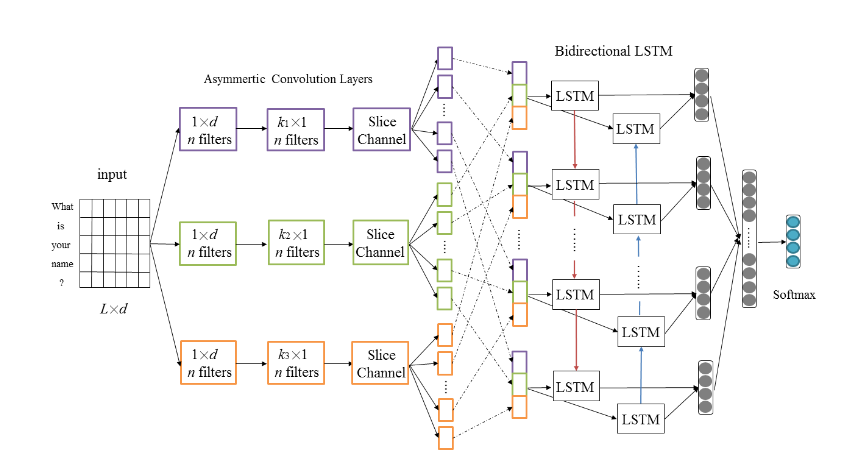
\includegraphics[scale=0.3]{./tex/natural-language-processing/acblstm.png}
\caption{Architecture de AC-BLSTM}
\label{acblstm}
\end{figure}

\begin{figure}
\centering
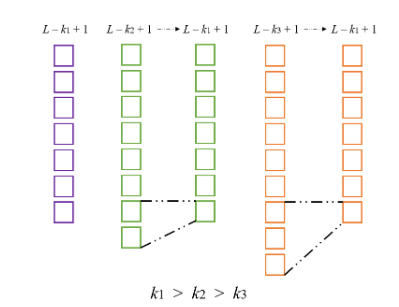
\includegraphics[scale=0.4]{./tex/natural-language-processing/acblsm2.png}
\caption{Harmonisation des dimensions des feature map selon l'approche de AC-BLSTM}
\label{acblstm2}
\end{figure}

\newpage
%\subsection{Traduction : Neural Machine Translation (NMT)}
%\noindent La plupart des problèmes de "séquence transduction" c'est à dire des taches qui transforme une séquence d'entrée en une séquence de sortie tels que les Neurals machine Translation utilisent à l'heure actuelle des modèles encodeur-décodeur utilisant des RNN (Recurrent Neural Network). L'idée est que l'encodeur va pouvoir construire des features sous forme de vecteurs qui représenteront au mieux notre séquence d'entrée (phrase/suite de mots). Le décodeur doit être capable d'interpréter au mieux cette représentation permettant ensuite de traduire notre séquence d'entrée dans la langue cible.
%\subsubsection{seq2seq}
%\subsubsection{convseq2seq}
%\subsubsection{Attention is all your need }
%\noindent \textbf{Attention Is All You Need} propose une approche utilisant également le concept d'encodeur-décodeur mais avec la particularité d'utiliser seulement un système de self attention avec une absence de CNN et RNN. Cela permet entre autre la parallélisation de calcul tout étant performant sur des séquences/dépendances longues portes. En effet, il est difficile de paralléliser des NMT utilisant des RNN puisqu'il est nécessaire de connaître l'état caché de l'instant précédent pour calculé celui de l'état caché de l'instant suivant. D'où l'architecture proposée appelée \textbf{Transformer}.\\

%\noindent Le Transformer est composé d'un encoder et d'un décodeur. Alors que la plupart des encodeurs/décodeurs pour les NMT empilent des RNNs tels que LSTMs ou GRUs, le Transformer va lui empiler des mécanismes de self-attention et de Feed Forward que ce soit au niveau de l'encodeur ou du décodeur. Le système de self-attention au niveau de l'encodeur compare grossièrement un mot de la séquence avec tous les autres mots et calcul leurs similarités. Cette opération est réalisée pour chaque mot de la séquence. Cela permet par exemple d'apprendre certaines relations/corrélations entre différents mots dans une phrase.
%\begin{figure}[H]
   % \centering
    %\includegraphics[scale=0.6]{NLP/AttentionIsAllYouNeed/SelfAttention.JPG}
    %\caption{Exemple de Self-Attention. Comme on peut le voir, le self attention permet d'obtenir des informations concernant la séquence d'entrées tels que la relation d'un mot dans la phrase. Dans cette exemple, "it" fait reference à "The animal".}
    %\label{ExSelfAttention}
%\end{figure}
%\noindent De plus, il est important de noter que le mécanisme d'attention est reproduit $h$ fois en parallèle (d'où l'appellation \textbf{Multi Head Attention}), ce qui permet d'avoir de multiples relations/corrélations pour un même mot.  Ces informations sont ensuite concaténées et encodées par un réseau FeedForward. Le vecteur de sortie de l'encodeur est ensuite transformé en set de deux vecteurs d'attentions qui seront utilisés par le décodeur afin de mieux se focaliser sur certaines parties de la séquence d'entrée du décodeur. Le décodeur va générer la traduction iterativement.

%\begin{figure}[H]
   % \includegraphics[scale=0.75]{NLP/AttentionIsAllYouNeed/transformer.jpg}
    %\caption{Architecture du Transformer.\\L'encodeur est composé de N$=$6 couches identique, dont chacune d'entre elle possède 2 sous couches. La première sous couches correspond à la "Multi Head Attention", alors que la seconde correspond à un position-wise Fully Connected Feed Forward. Afin de mieux repropager le gradient lors de l'apprenttisage et pour rendre le modèle plus stable,une connexion résiduel et une couche de normalization est appliqué à la fin de chaque sous couche.  Pour faciliter les connections résiduels, toutes les sous couches du model ont une entrée et une sortie de dimension $d_{model}$ $=$ 512. De même, le décodeur est composé de N=6 couches identiques. Cependant, ce dernier possède une sous couches en plus : "Masked Multi Head Attention". L'utilisation des résidus et des couches de normalisations est identique.}
   % \label{ArchTransformer}
%\end{figure}

%\noindent Ainsi, détaillons un peu plus le système d'attention et quelques briques du modèle :
%\textbf{Embedding et Positional Encoding} : Comme dans la plupart de ce genre de modèle, les séquences d"entrées sont décomposées en tokens qui sont ensuite modélisées en vecteur de dimension $d_{model}$ $=$ 512. \\
%\noindent On peut noter l'utilisation du "positional encoding". En effet, comme le modèle n'utilise ni de RNN, ni de CNN l'ordre dans la séquence n'est pas indiqué. Par conséquent, il est utile d'ajouter cette information au niveau des embeddings. Le "positional encoding" a la même dimension que l'embedding d'entrée/sortie soit $d_{model}$. Par conséquent, il suffit de sommer les deux vecteurs. La méthode proposé par \textbf{Attention Is All you Need} pour calculer le  "positional encoding" est d'utilisé la fonction sinus et cosinus tels que : \\
%$$PE_{(pos, 2i)} = sin(pos/10000^{2i/d_{model}})$$\\
%$$PE_{(pos, 2i+1)} = cos(pos/10000^{2i/d_{model}})\, avec\, pos \,  la \,  position, i \, la \, dimension.$$ \\
%\noindent L'hypothèse est qu'il est facile d'apprendre une position relative avec cette formulation, similaire à des signaux puisqu'il est facile d'écrire $PE_{pos+k}$ en fonction de $PE_{pos}$ de façon linéaire.\\

%\noindent Lors du décodage de la sortie, pour prédire la probabilité du token suivant  , une fonction softmax est utilisé. Les poids des embeddings sont multipliés par un facteur $\sqrt{d_{model}}$ avant le calcul de softmax. (question pratique pour ne pas avoir de valeurs trop petite)\\\\
%\noindent \textbf{Multi Head attention} :
%\noindent L'entrée de ce module est caractérisé par 3 types de vecteurs qui sont une "query" : Q (dimension $d_v$) et une "key" : K et une "value" : V (dimension $d_k$) pour CHAQUE mot/représentation de mot. Si notre séquence est de longueur L, nous aurons L vecteurs "query" Q, L vecteurs "key" K et L vecteurs "value" V. Pour calculer la comparaison mentionnée précédemment, on utilise le module \textbf{Scaled Dot Product Attention} dans lequel on multiplie chaque query Q avec toutes les keys K. Ainsi, pour chaque query nous obtenons L nouveaux vecteurs que l'on "normalise" en divisant par la $\sqrt{d_k}$ afin de réduire les valeurs lorsqu'elles sont trop grandes (notamment pour une stabilité du calcul de gradient). On applique ensuite un softmax qui permet d'obtenir l'importance de chaque mot dans la séquence par rapport à la query. On multiplie ensuite par le vecteur V correspondant aux différents mots de notre séquence, ainsi les mots ayant une faible relation avec la query(qui est également la représentation d'un mot) auront leurs valeurs diminuées.\\
%\noindent "Linear", avant le Scale Dot Product attention, correspond à une matrice $W^Q$/$W^K$/$W^V$ permettant de passer des données d'entrées de dimension Lx$d_{model}$ à Lx$d_k$ ou Lx$d_v$. En effet la dimension à l'entrée et sortie de chaque sous couche est fixé $d_{model}$ $=$ 512.\\
%\noindent En pratique, pour des raisons de parallélisation, on utilise des matrices au lieu d'utiliser des vecteurs. C'est à dire que que tous les Q sont dans une seul matrice de dimension $L$x $d_v$, de même pour K et V avec pour chacun d'entre eux une matrice de dimension $L$x $d_k$.\\
%$$Attention(Q, K, V)\, =\, softmax(\frac{QK^T}{\sqrt{d_k}})V$$\\
%\noindent De plus, au lieu de calculer une seul fonction d'attention de dimension $d_{model}$ pour "key", "value", "query", il semble plus efficace de calculer h fonction de self-attention avec $d_k$ dimension pour "key" et "value", $d_v$ dimension pour "query" tels que hx$d_v$ $=$ hx$d_k$ $=$ $d_{model}$. Les h fonction d'attention peuvent ainsi être calculé en parallèle. Les h sorties sont ensuite concatenée et on multiplie par une matrice $W^{O}$ de dimension h$d_v$x$d_{model}$ afin d'obtenir une dimension $d_{model}$. L'hypothese est que calculer de multiple fois les fonctions de self-attention (avec donc des poids differents) permet d'obtenir différentes relations/corrélations/informations que l'on aurait pas avec une seul. \\
%$$MultiHead(Q, K, V)\, =\, Concat(head_1, ... head_h)W^O$$ \\
%$$avec\: head_i  \,=\, Attention(QW^Q_i, KW^K_i, VW^V_i)$$ \\
%cette fonction d'attention peut être décrit comme la modélisation d'une "query" :Q (dimension $d_v$) et d'une paire "key":K et "value":V (dimension $d_k$) qui sont tous les 3 des vecteurs. Si notre séquence est de longueur L, nous aurons L vecteurs "query", L vecteurs "key" et L vecteurs "value". \\
%Dans le cas du décodeur, la "query" provient de la couche précédente du décodeur, alors que "key" et "value" proviennent de la sortie de l'encodeur. Dans le cas de l'encodeur (et du décodeur pour le "Masked Multi Head attention"), ces 3 vecteurs proviennent des couches précédentes. (voir Figure \ref{ArchTransformer}) \\La sortie de cette fonction correspond au produit de la "query" Q avec toutes les "keys" K auquel on divise par $\sqrt{d_k}$ afin de réduire les valeurs lorsqu'elles sont trop grandes (notamment pour une stabilité du calcul de gradient). On applique ensuite un softmax. Ce calcul de self-attention permet par exemple de voir certaines relations, ou information utile entre les mots/entités de la séquence. (Figure \ref{ExSelfAttention})


%\noindent On multiplie ensuite par le vecteur V. Tout ce calcul est appelé "Scaled Dot-Product Attention". En pratique, Q , V et K sont des matrices et non des vecteurs afin de faire du calcul en parallèle. En effet, la fonction expliqué ci dessus s'applique pour un(e) seule entité/mot de notre séquence. Dans le cas d'une séquence tels une phrase, les entités seront des mots. Pour une question d'optimisation de temps, on utilisera des produits matriciels au lieu de produit simple permettant de calculer la fonction d'attention sur toute la séquence. (d'où la transposé)



%\noindent \textbf{Position-wise Fully Connected Network} : ce dernier repose sur un MLP à deux couches qui possède une fonction d'activation RELU entre les deux couches. La dimension d'entrée et de sortie est $d_{model}$ $=$512. La couche interne possède 2048 neurones. On peut également voir le MLP comme un CNN de kernel 1. On peut considérer qu'il permet d'encoder l'information basé sur l'attention de la sous couche précédente.  \\\\
%\noindent \textbf{Mask Multi Head attention} : Similaire à la couche Multi Head Attention avec la différence qu'un masque avec des valeurs valant -$\infty$ est appliqué à partir d'un certain indice car certaines valeurs/prédictions au niveau du décodeur n'ont pas encore été calculé.
